% !TeX root = ../main.tex

\begin{frame}
  \frametitle{Overview: The Geometric Case}

  \begin{textblock*}{11cm}(1cm,2cm)
    Unknown $c$-Lipschitz function $f : D\to \R$.\vspace{1ex}

    \only<2,3>{Finite sample $P\subset D$ of $f$.\vspace{1ex}}

    \only<3>{Coverage radius $\delta > 0$, covered region $P^\delta$.}
  \end{textblock*}

  \begin{textblock*}{12cm}(0.5cm,5cm)
    \includegraphics<1>[trim=50 200 50 200, clip, width=0.45\textwidth]{figures/nbhd/D}%
    \includegraphics<2>[trim=50 200 50 200, clip, width=0.45\textwidth]{figures/nbhd/P}%
    \includegraphics<3>[trim=50 200 50 200, clip, width=0.45\textwidth]{figures/nbhd/CP}
  \end{textblock*}
\end{frame}

\begin{frame}
  \frametitle{Overview: The Geometric Case}

  \begin{textblock*}{11cm}(1cm,2cm)
    Sublevel set $B_\omega$ that surrounds $D$.\vspace{1ex}

    \only<2,3>{Sample $Q$ such that $Q^\delta\subseteq B_\omega$\vspace{1ex}}

    \only<3>{For $\zeta \geq \delta$ set $Q = P\cap B_{\omega-c\zeta}$}
  \end{textblock*}

  \begin{textblock*}{12cm}(0.5cm,5cm)
    \includegraphics<1>[trim=50 200 50 200, clip, width=0.45\textwidth]{figures/nbhd/B0}%
    \includegraphics<2>[trim=50 200 50 200, clip, width=0.45\textwidth]{figures/nbhd/Q0}%
    \includegraphics<3>[trim=50 200 50 200, clip, width=0.45\textwidth]{figures/nbhd/CQ0}
  \end{textblock*}
\end{frame}

\begin{frame}
  \frametitle{Overview: The Geometric Case}
  \begin{textblock*}{11cm}(1cm,2cm)
    \begin{small}
    \begin{description}
      \item[Goal:] Show $\ell : \hom_0(\overline{B_\omega}, \overline{D})\to \hom_0(\overline{Q^\delta},\overline{P^\delta})$ is injective
      \item[Method:] Check $\mathbf{dim}~\hom_0(D\setminus B_\omega)\leq \mathbf{dim}~\hom_0(\overline{Q^\delta}, \overline{P^\delta})$
      \item[Problem:] Possible $\mathbf{dim}~\hom_0(D\setminus B_\omega)\leq \mathbf{dim}~\hom_0(\overline{Q^\delta}, \overline{P^\delta})$ and $\ell$ is not injective.
      \item<7>[Solution:] Choose $Q_0, Q_1\subset P$ such that $\mathbf{dim}~\hom_0(D\setminus B_\omega)\geq \mathbf{rk}~\hom_0((\overline{Q_1^\delta}, \overline{P^\delta})\hookrightarrow(\overline{Q_0^\delta}, \overline{P^\delta}))$.
    \end{description}
    \end{small}
  \end{textblock*}

  \begin{textblock*}{12cm}(0.75cm,5.5cm)
    \includegraphics<2,3>[trim=50 250 50 300, clip, width=0.4\textwidth]{figures/ass1/surf}%
    \includegraphics<4,5>[trim=50 250 50 300, clip, width=0.4\textwidth]{figures/ass1/DBcomp}%
    \includegraphics<6>[trim=50 250 50 300, clip, width=0.4\textwidth]{figures/ass1/Bint}\hspace{6ex}%
    \includegraphics<3>[trim=50 250 50 300, clip, width=0.4\textwidth]{figures/ass1/full}%
    \includegraphics<4>[trim=50 250 50 300, clip, width=0.4\textwidth]{figures/ass1/PQcomp}%
    \includegraphics<5>[trim=50 250 50 300, clip, width=0.4\textwidth]{figures/ass1/PQcomp-spread}%
    \includegraphics<6>[trim=50 250 50 300, clip, width=0.4\textwidth]{figures/ass1/Qint}
  \end{textblock*}
\end{frame}

\begin{frame}
  \frametitle{Overview: The Geometric Case}
  \begin{textblock*}{11cm}(1cm,2cm)
  \begin{small}
    Let $Q_0 = P\cap B_{\omega-c\zeta}$ and $Q_1 = P\cap B_{\omega+c\delta}$\vspace{1ex}

    Let $i : \hom_0(\overline{Q_1^\delta}, \overline{P^\delta})\to \hom_0(\overline{Q_0^\delta}, \overline{P^\delta})$.

    \only<2>{\begin{lemma}\label{lem:psurj}
        If $B_\omega$ surrounds $D$ in $\X$ then $\mathbf{dim}~\hom_0(D\setminus B_\omega)\geq \mathbf{rk}~i$.
    \end{lemma}}
  \end{small}
  \end{textblock*}

  \begin{textblock*}{12cm}(0.75cm,5.5cm)
    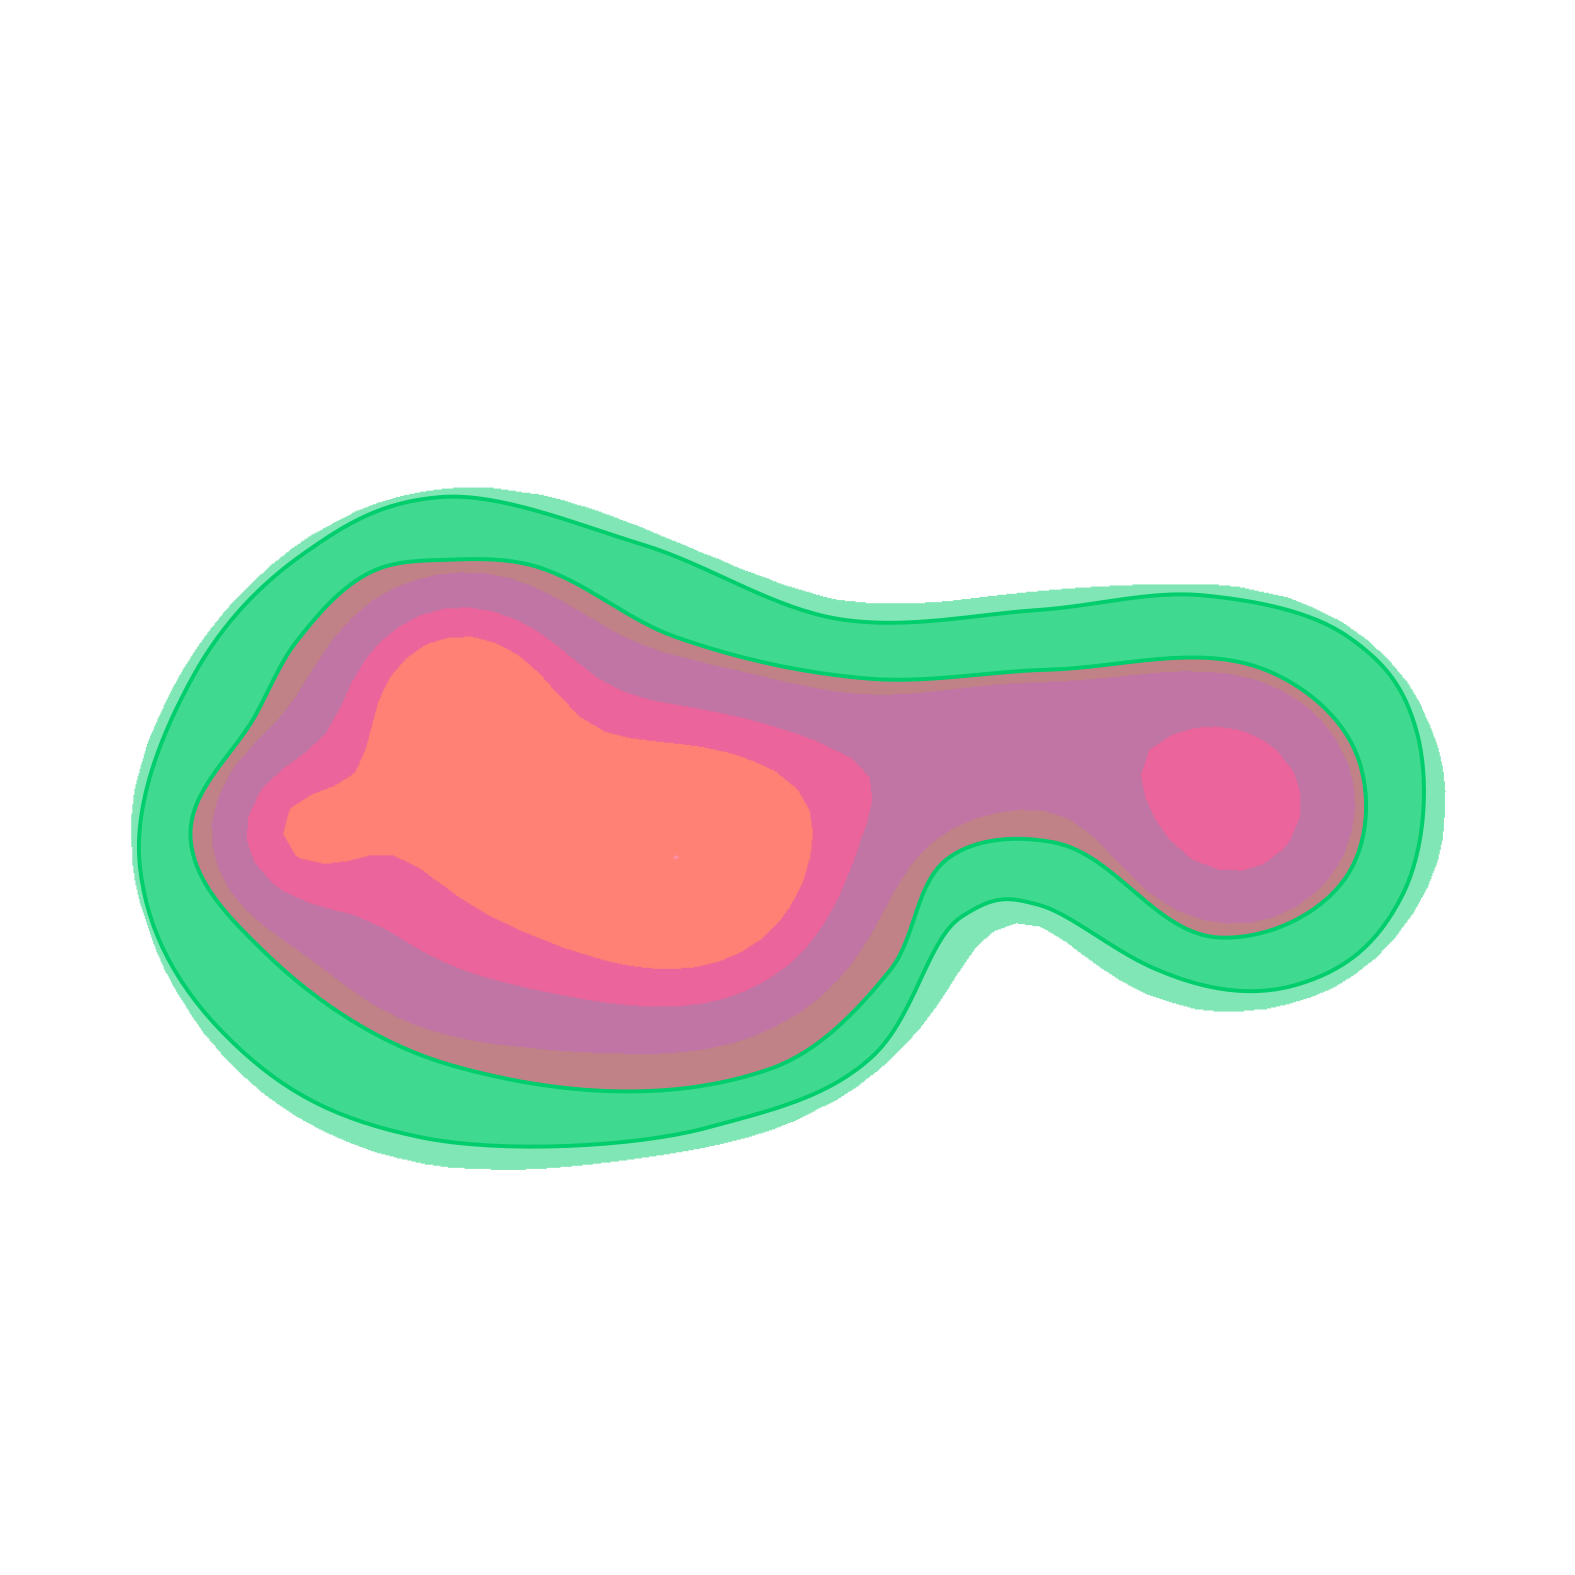
\includegraphics[trim=50 250 50 300, clip, width=0.4\textwidth]{figures/nbhd/PQ0}\hspace{6ex}%
    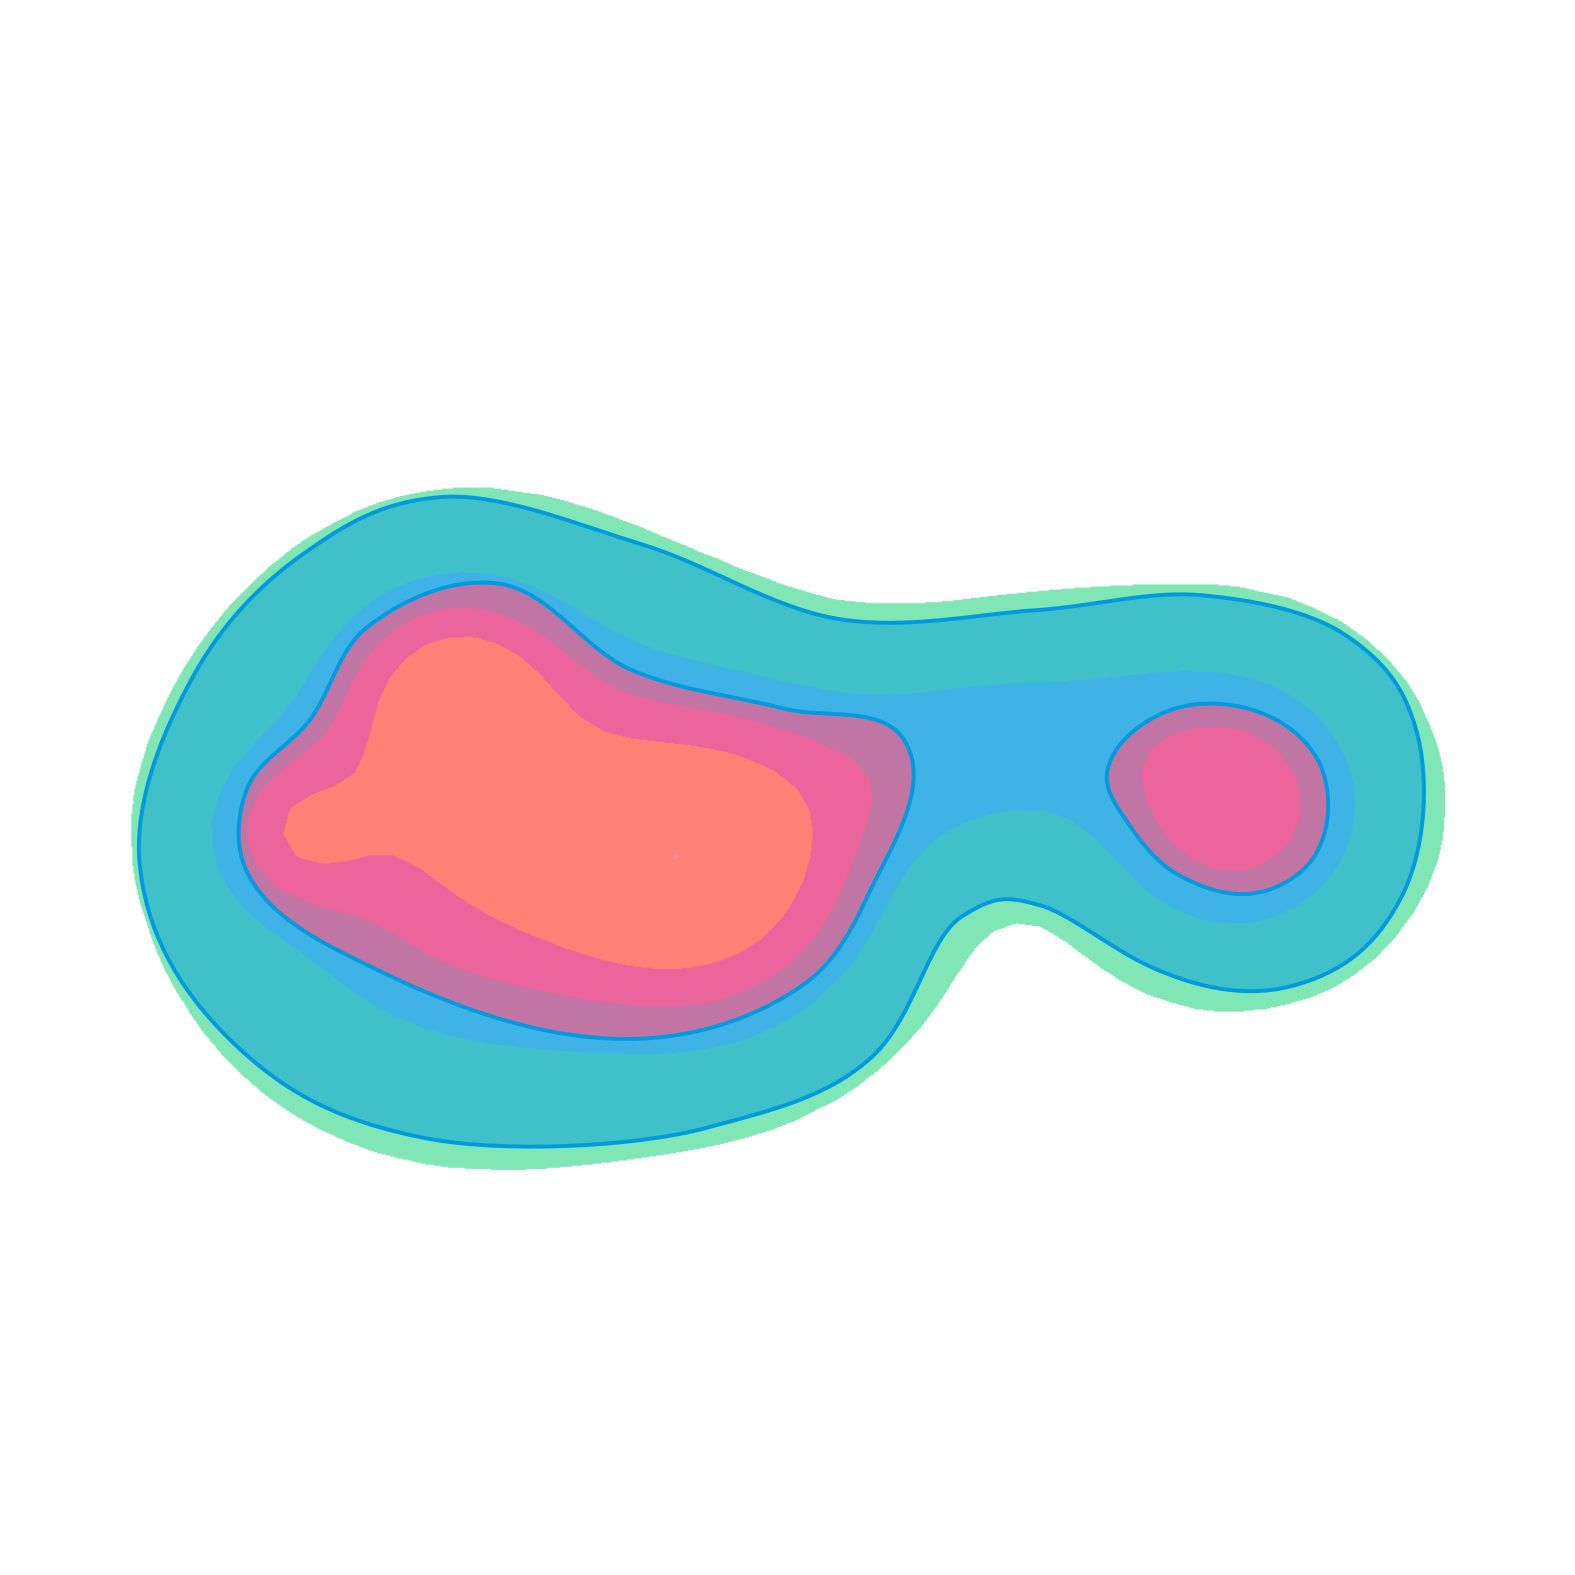
\includegraphics[trim=50 250 50 300, clip, width=0.4\textwidth]{figures/nbhd/PQ1}
  \end{textblock*}
\end{frame}

\begin{frame}
  \frametitle{{\small Assumption 1 and the Geometric TCC}}

  \begin{textblock*}{11cm}(1cm,2cm)
    Recall $\ell$ must be induced by inclusion.\vspace{1ex}

    Let $B_1 = B_{\omega+2c\delta}$ so $Q_1^\delta\subseteq B_1$.\vspace{1ex}
  \end{textblock*}

  \begin{textblock*}{11cm}(1cm,4.5cm)
    \only<1>{\[\begin{tikzcd}[ampersand replacement=\&]
      (P^\delta, Q_0^\delta) \arrow[hookrightarrow]{r}\arrow[hookrightarrow]{d} \&
      (P^\delta, Q_1^\delta) \arrow[hookrightarrow]{d} \\
      %
      (D, B_\omega) \arrow[hookrightarrow]{r} \&
      (D, B_1)
    \end{tikzcd}\]}

    \only<2>{\[\begin{tikzcd}[ampersand replacement=\&]
      \hom_0(\overline{B_1},\overline{D})\arrow{d}{m} \arrow{r}{j} \&
      \hom_0(\overline{B_\omega}, \overline{D}) \arrow{d}{\ell} \\
      %
      \hom_0(\overline{Q_1^\delta}, \overline{P^\delta}) \arrow{r}{i} \&
      \hom_0(\overline{Q_0^\delta}, \overline{P^\delta}).
    \end{tikzcd}\]}
  \end{textblock*}
\end{frame}

\begin{frame}
  \frametitle{{\small Assumption 1 and the Geometric TCC}}

  \begin{textblock*}{11cm}(1cm,2cm)
    \begin{small}
      \begin{description}
        \item[Assumption 1] $j : \hom_0(D\setminus B_{1}\hookrightarrow D\setminus B_\omega)$ is \emph{surjective}.
      \end{description}

      \only<2>{Now, $\mathbf{rk}~j = \mathbf{dim}~\hom_0(D\setminus B_\omega)$.}
    \end{small}
  \end{textblock*}

  \begin{textblock*}{11cm}(1cm,5cm)
    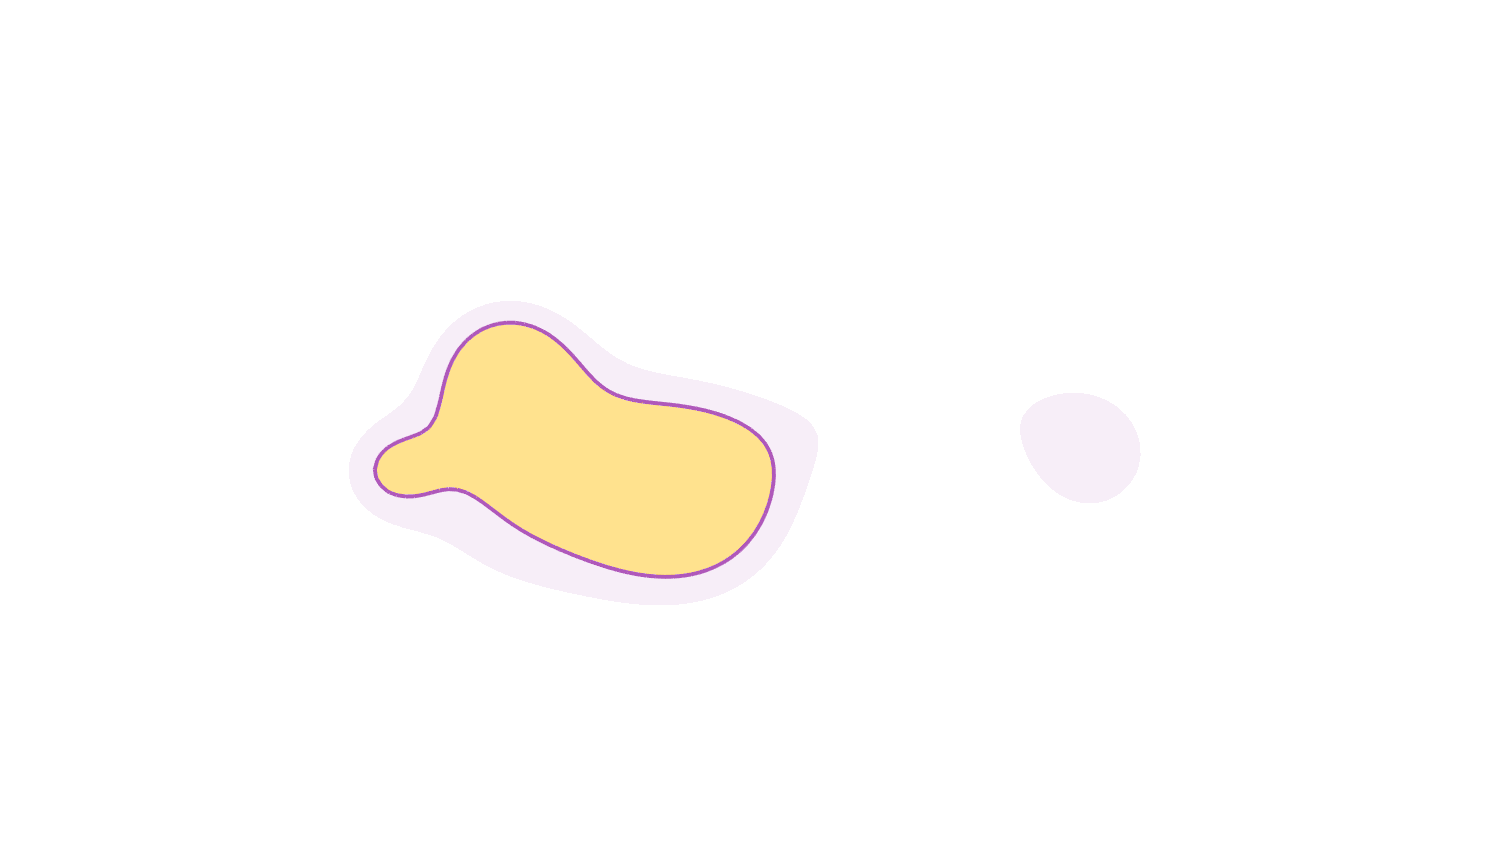
\includegraphics[trim=300 150 200 200, clip, width=0.4\textwidth]{../scripts/figures/surf/ass1_D_top.png}\hspace{6ex}
    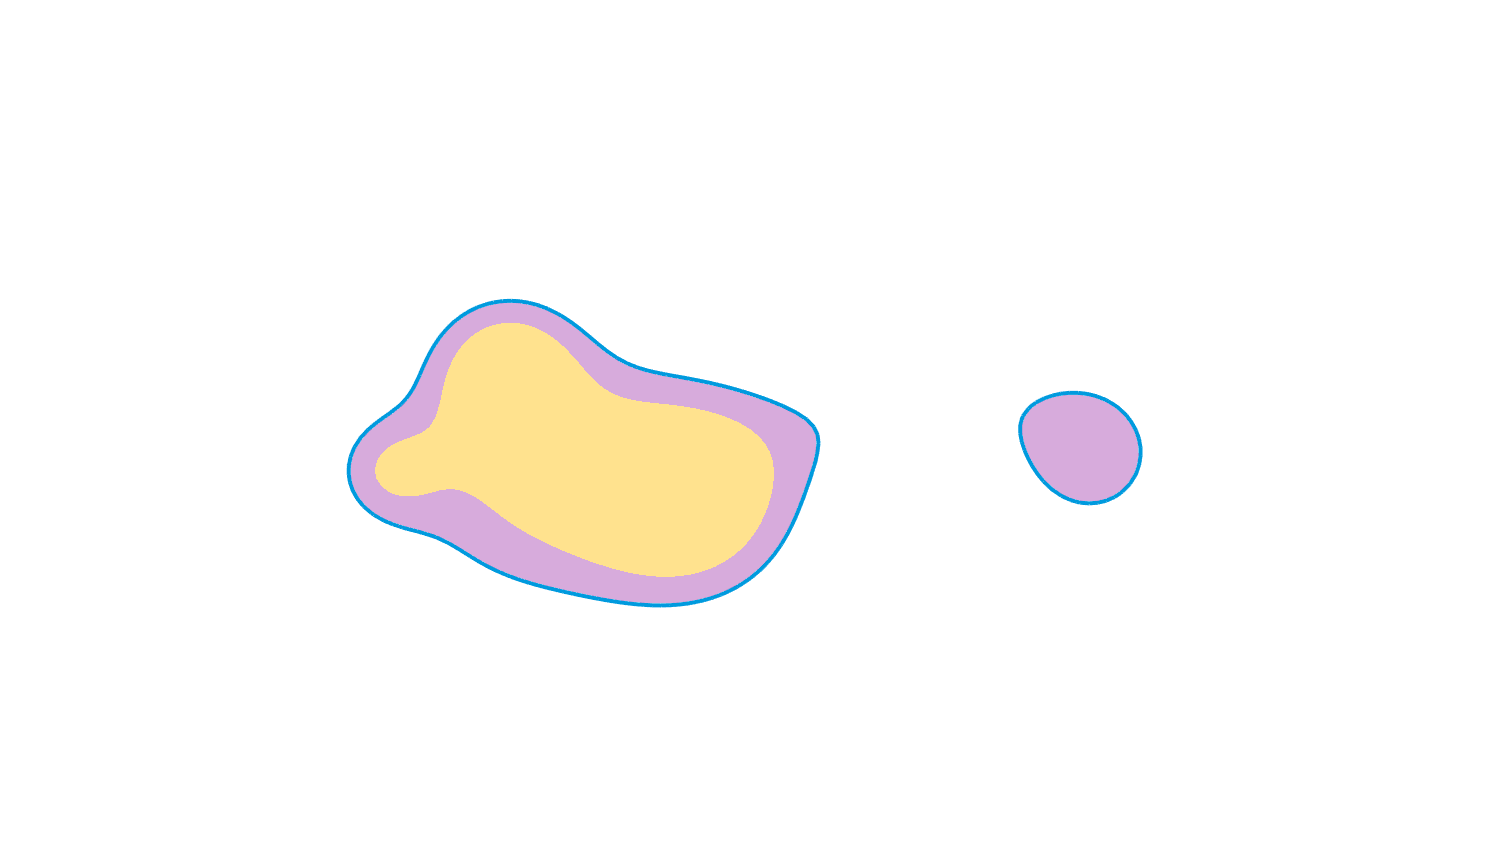
\includegraphics[trim=300 150 200 200, clip, width=0.4\textwidth]{../scripts/figures/surf/ass1_C_top.png}
  \end{textblock*}

  % \begin{textblock*}{11cm}(1cm,4.5cm)
  %   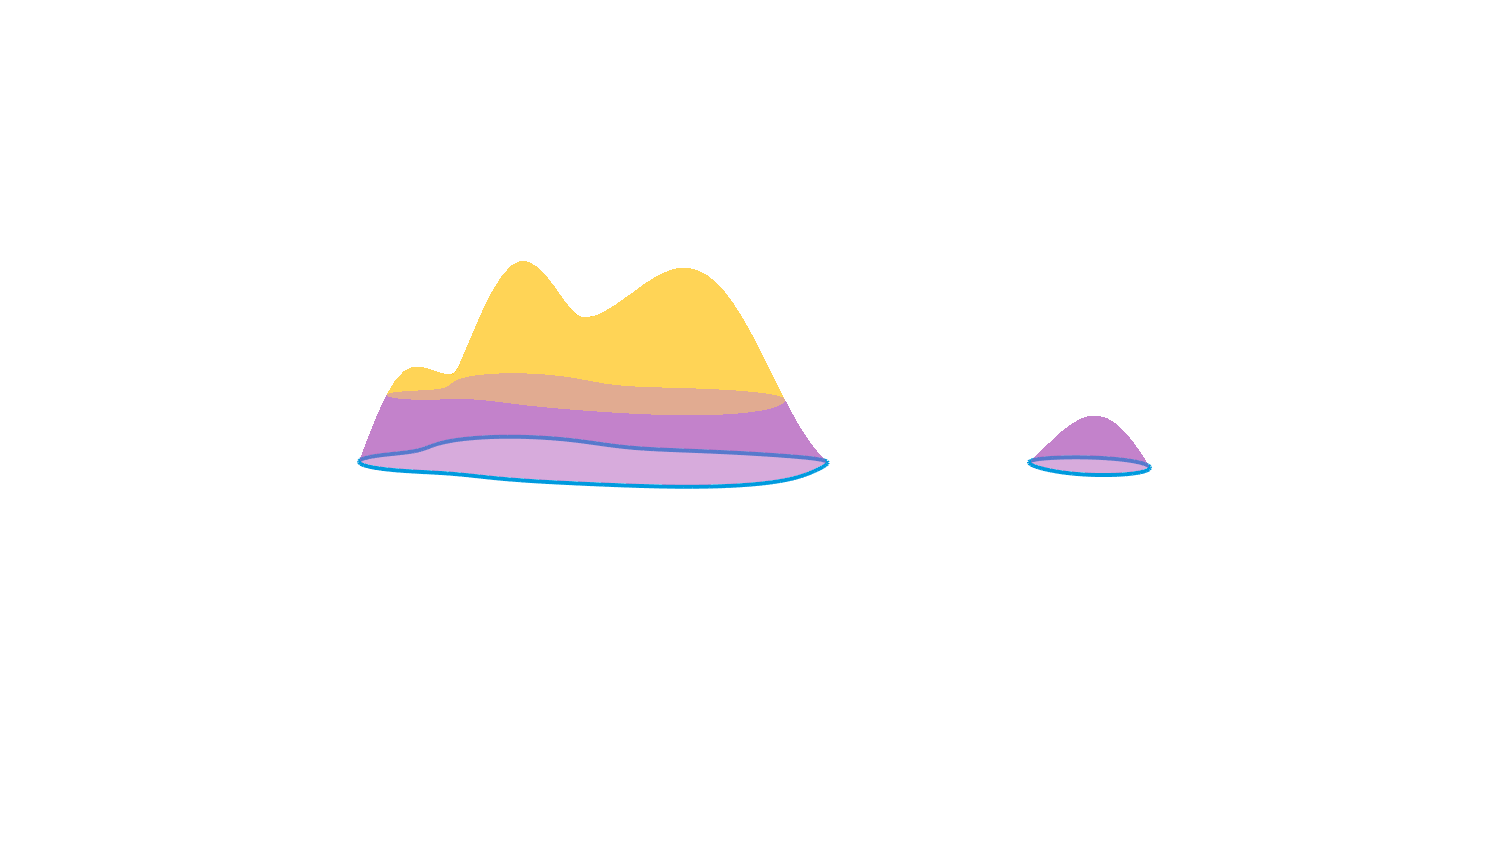
\includegraphics[trim=200 300 200 200, clip, width=0.5\textwidth]{../scripts/figures/surf/ass1_C_side.png}%
  %   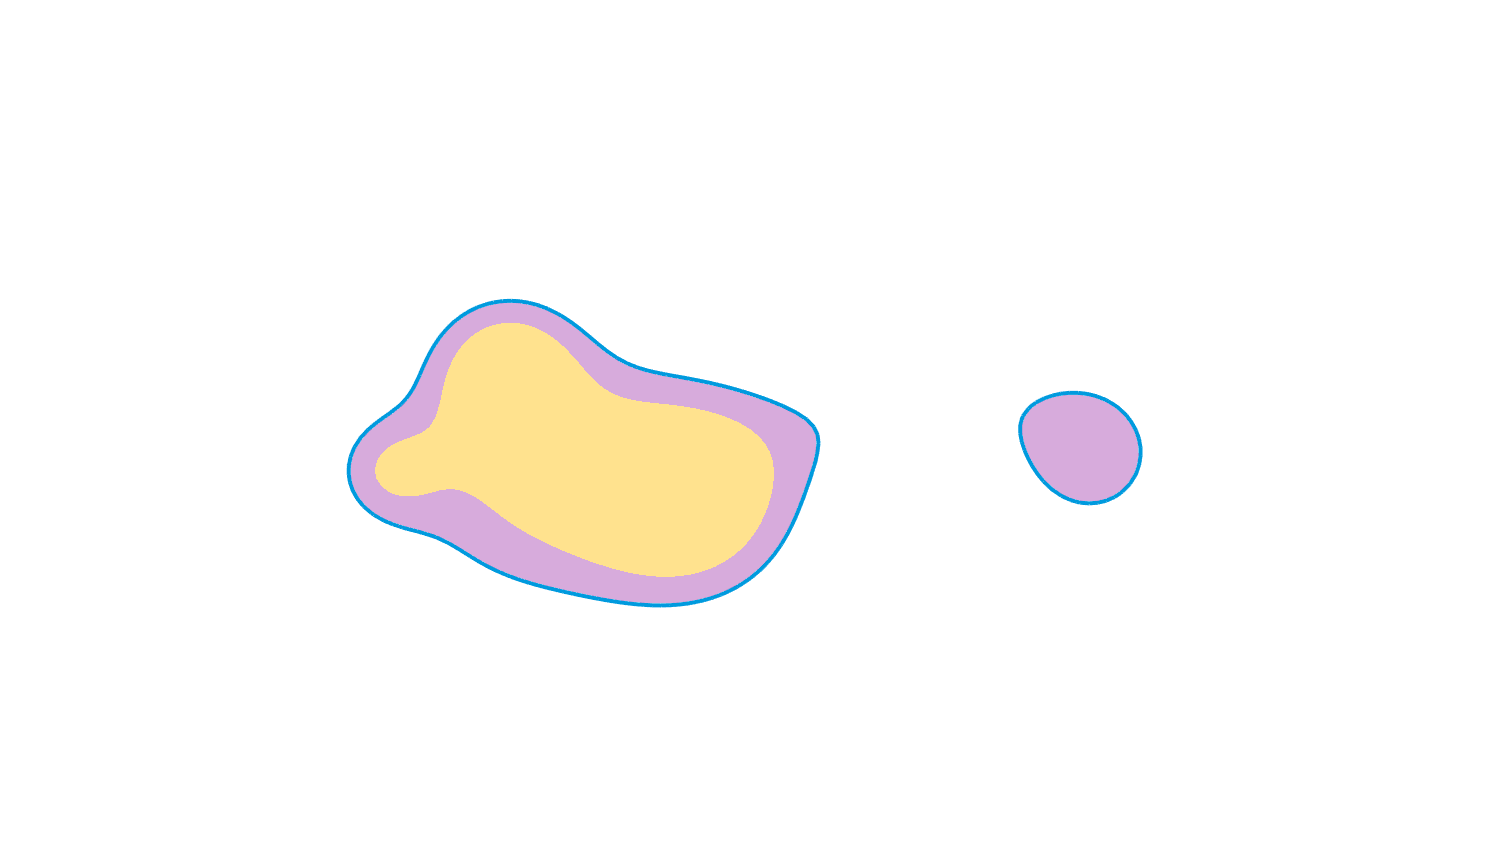
\includegraphics[trim=300 150 200 200, clip, width=0.3\textwidth]{../scripts/figures/surf/ass1_C_top.png}\\%
  %   
\includegraphics[trim=200 300 200 200, clip, width=0.5\textwidth]{../scripts/figures/surf/ass1_D_side.png}%
  %   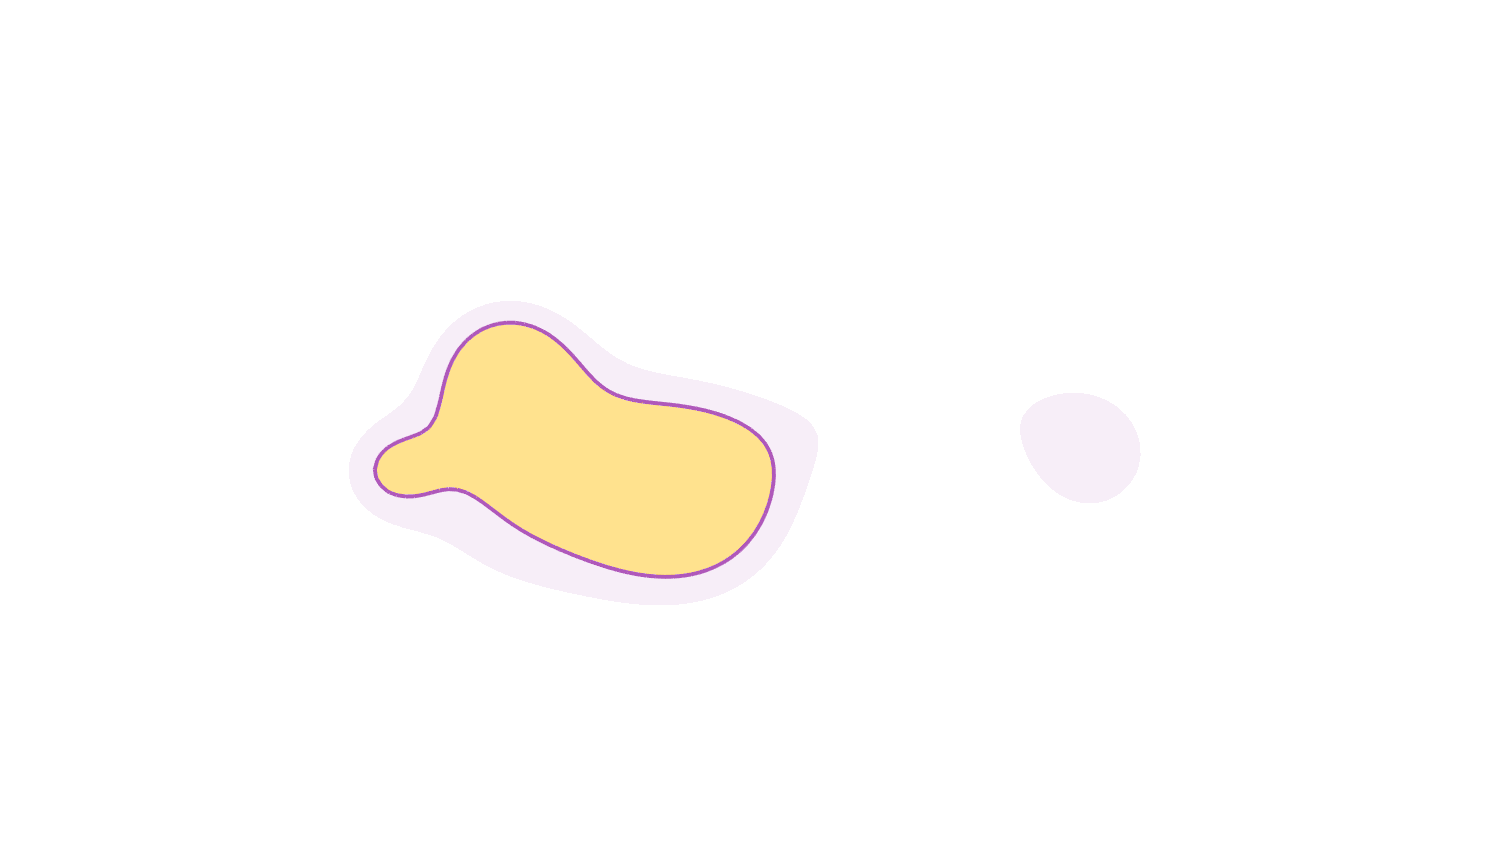
\includegraphics[trim=300 150 200 200, clip, width=0.3\textwidth]{../scripts/figures/surf/ass1_D_top.png}
  % \end{textblock*}
\end{frame}


\begin{frame}
  \frametitle{{\small Assumption 1 and the Geometric TCC}}

  \begin{textblock*}{11cm}(1cm,2cm)
    \begin{small}\begin{theorem}[Geometric TCC]
        If $j$ is surjective and $\mathbf{rk}~i\geq \mathbf{rk}~j$ then $D\setminus B_\omega\subseteq P^\delta$ and $Q_0^\delta$ surrounds $P^\delta$ in $D$.
    \end{theorem}\end{small}
  \end{textblock*}

  \begin{textblock*}{11cm}(1cm,4.5cm)
    \[\begin{tikzcd}[ampersand replacement=\&]
      \hom_0(\overline{B_1},\overline{D})\arrow{d}{m} \arrow{r}{j} \&
      \hom_0(\overline{B_\omega}, \overline{D}) \arrow{d}{\ell} \\
      %
      \hom_0(\overline{Q_1^\delta}, \overline{P^\delta}) \arrow{r}{i} \&
      \hom_0(\overline{Q_0^\delta}, \overline{P^\delta}).
    \end{tikzcd}\]
  \end{textblock*}
\end{frame}

% \begin{frame}
%   \frametitle{Overview: Main Theorems}
%
%   \begin{textblock*}{11cm}(1cm,2cm)
%     \begin{small}\begin{theorem}[Geometric TCC]
%         If
%         \[ \mathbf{rk}~\hom_0((\overline{Q_1^\delta},\overline{P^\delta})\hookrightarrow (\overline{Q_0^\delta},\overline{P^\delta}))\geq \mathbf{dim}~\hom_0(D\setminus B_\omega)\]
%         then $D\setminus B_\omega\subseteq P^\delta$ and $Q_0^\delta$ surrounds $P^\delta$ in $D$.
%     \end{theorem}\end{small}
%   \end{textblock*}
%
%   \begin{textblock*}{11cm}(1cm,5cm)
%     \only<2>{\begin{small}\begin{theorem}[Algorithmic TCC]
%         If
%         \[ \mathbf{rk}~\hom_d(\rips^\delta(P,Q_0)\hookrightarrow \rips^{2\delta}(P, Q_1))\geq \mathbf{dim}~\hom_0(\rips^\delta(P\setminus Q_{0}))\]
%         then $D\setminus B_\omega\subseteq P^\delta$ and $Q_0^\delta$ surrounds $P^\delta$ in $D$.
%     \end{theorem}\end{small}}
%   \end{textblock*}
%
% \end{frame}
